%\documentclass[a4paper]{jarticle} 
\documentclass[dvipdfmx,a4paper]{jsarticle}
\usepackage{tikz}
\usepackage{amsmath}
\usepackage{amssymb}
\topmargin = 0mm
\oddsidemargin = 5mm
\textwidth = 152mm
\textheight = 240mm


% サブセクションを 問1,問2 にする設定
\renewcommand{\thesection}{[\arabic{section}]}

% サブサブセクションを (1),(2)にする設定
\renewcommand{\thesubsection}{(\arabic{subsection})}
% (i),(ii)なら \arabic を \roman に変える。    (a),(b)なら \alph

\renewcommand{\thesubsubsection}{(\roman{subsubsection})}

% 大問2の3番目の計算式のラベルを (2.3) にする設定
% 計算式の参照には \eqref{eq:hoge} を使う
\makeatletter
  \renewcommand{\theequation}{\arabic{subsection}.\arabic{equation}}
  \@addtoreset{equation}{subsection}
\makeatother

% --------------------------------------------------------------------
\begin{document}

% タイトル
\begin{center}
\textbf{\huge{数学2D演習 第6回}}
\end{center}

%名前
\begin{flushright}
工学部電気電子工学科3年 03200489 末吉七海\\
\end{flushright}

% --------------------------------------------------------------------
% [1]
\section{復習}

%(1)
\subsection{$\mbox{\Large$\oint_{|z| = 1}\frac{\mathrm{d}z}{3z^2-5z-2}$}$}
$\mbox{\Large$\frac{1}{3z^2-5z-2}$}$の極で積分経路にの内側にあるものは、 $z = -\mbox{\large$\frac{1}{3}$}$\\
$z = -\mbox{\large$\frac{1}{3}$}$における留数は、
\begin{align*}
Res\biggl(\frac{1}{3z^2-5z-2}, z = -\frac{1}{3}\biggr) &= \lim_{z \to -\frac{1}{3}} \Bigl(\bigl(z - \frac{1}{3}\bigr)\frac{1}{3z^2-5z-2}\Bigr)\\
&=\lim_{z \to -\frac{1}{3}} \frac{1}{3(z-2)}\\
&=-\frac{1}{7}
\end{align*}
よって、
\begin{align*}
\oint_{|z| = 1}\frac{\mathrm{d}z}{3z^2-5z-2} =- \frac{2\pi i}{7}
\end{align*}
\\

%(2)
\subsection{$\mbox{\Large$\int_{0}^{2\pi}\frac{\mathrm{d}\theta}{5\cos{\theta} - 13}$}$}
$e^{i\theta} = z$と置換すると、$\mbox{\large$\frac{1}{iz}$}\mathrm{d}\theta = \mathrm{d}z$
\begin{align*}
\int_{0}^{2\pi}\frac{\mathrm{d}\theta}{5\cos{\theta} - 13} &= \oint_{|z| = 1}\frac{\mathrm{d}z}{iz(5\frac{z + z^{-1}}{2} - 13)}\\
&= \frac{2}{i}\oint_{|z| = 1}\frac{\mathrm{d}z}{5z^2 - 26z + 5}
\end{align*}
積分経路の内側にある$\mbox{\large$\frac{1}{5z^2 - 26z + 5}$}$の極は、$z = \mbox{\large$\frac{1}{5}$}$\\
$z = \mbox{\large$\frac{1}{5}$}$における留数は、
\begin{align*}
Res\biggl(\frac{1}{5z^2 - 26z + 5}, z = \frac{1}{5}\biggr) &= \lim_{z\to \frac{1}{5}}\biggl(\bigl(z - \frac{1}{5}\bigr)\frac{1}{5z^2 - 26z + 5}\biggr)\\
&= \lim_{z\to \frac{1}{5}}\frac{1}{5(z-5)}\\
&=-\frac{1}{24}
\end{align*}
よって、
\begin{align*}
\int_{0}^{2\pi}\frac{\mathrm{d}\theta}{5\cos{\theta} - 13} &= \frac{2}{i}\oint_{|z| = 1}\frac{\mathrm{d}z}{5z^2 - 26z + 5} \\
&= \frac{2}{i} \times 2\pi i \times \bigl(-\frac{1}{24}\bigr)\\
&= -\frac{\pi}{6}
\end{align*}
\\

%(3)
\subsection{$\mbox{\Large$\int_{0}^{2\pi}\frac{\mathrm{d}\theta}{\sin{\theta} + 2}$}$}
$e^{i\theta} = z$と置換すると、$\mbox{\large$\frac{1}{iz}$}\mathrm{d}\theta = \mathrm{d}z$
\begin{align*}
\int_{0}^{2\pi}\frac{\mathrm{d}\theta}{\sin{\theta} + 2} &= \oint_{|z| = 1}\frac{\mathrm{d}z}{iz(\frac{z - z^{-1}}{2i} + 2)}\\
&= 2\oint_{|z| = 1}\frac{\mathrm{d}z}{z^2 + 4iz - 1}
\end{align*}
積分経路の内側にある$\mbox{\large$\frac{1}{z^2 + 4iz - 1}$}$の極は、$z = -2i + \sqrt{3}i$\\
$z = -2i + \sqrt{3}i$における留数は、
\begin{align*}
Res\biggl(\frac{1}{z^2 + 4iz - 1}, z = -2i + \sqrt{3}i\biggr) &= \lim_{z\to -2i + \sqrt{3}i}\biggl(\bigl(z - (-2i + \sqrt{3}i)\bigr)\frac{1}{z^2 + 4iz - 1}\biggr)\\
&= \lim_{z\to -2i + \sqrt{3}i}\frac{1}{z - (-2i - \sqrt{3}i)}\\
&= \frac{1}{-2i + \sqrt{3}i - (-2i - \sqrt{3}i)}\\
&=\frac{1}{2\sqrt{3}i}
\end{align*}
よって、
\begin{align*}
\int_{0}^{2\pi}\frac{\mathrm{d}\theta}{\sin{\theta} + 2} &= 2\oint_{|z| = 1}\frac{\mathrm{d}z}{z^2 + 4iz - 1}\\
&= 2 \times 2\pi i \times \frac{1}{2\sqrt{3}i}\\
&= \frac{2\sqrt{3}\pi}{3}
\end{align*}
\\\\

%[2]
\section{ラプラス方程式の境界値問題}
%(1)
\subsection{}
$z = x + iy \to f(z) = \xi(x,y) + \eta(x,y)$という等角写像を考える。\\
以下においては、$\partial_x\xi = \xi_x$のように表すとする。\\
$f(z) = \xi(x,y) + \eta(x,y)$は正則より、CR方程式が成り立ち、
\begin{eqnarray}
\label{1}
\xi_x &= \eta_y\quad
\xi_y = -\eta_x\\
\therefore\quad\xi_{xx} &= \eta_{yx}\quad
\xi_{yy} = -\eta_{xy}\nonumber\\
\xi_{xy} &= \eta_{yy}\quad
\xi_{yx} = -\eta_{xx}\nonumber
\end{eqnarray}
よって、
\begin{equation}
\label{2}
\xi_{xx} + \xi_{yy} = 0\quad\eta_{xx} + \eta_{yy} = 0
\end{equation}
$f(z) = \xi(x,y) + \eta(x,y)$のから、
\begin{align*}
\partial_x = \xi_x\partial_\xi + \eta_x\partial_\eta\\
\partial_y = \xi_y\partial_\xi + \eta_y\partial_\eta
\end{align*}
さらにそれぞれの式を、$x, y$で微分すると、
\begin{align*}
\partial_x^2 &= \xi_{xx}\partial_\xi + \xi_x\partial_x\partial_\xi + \eta_{xx}\partial_\eta + \eta_x\partial_x\partial_\eta\\
&=\xi_{xx}\partial_\xi + \xi_x(\xi_x\partial_\xi + \eta_x\partial_\eta)\partial_\xi + \eta_{xx}\partial_\eta + \eta_x(\xi_x\partial_\xi + \eta_x\partial_\eta)\partial_\eta\\
&=\xi_{xx}\partial_\xi + \xi_x^2\partial_{\xi\xi} + \xi_x\eta_x\partial_{\eta\xi} + \eta_{xx}\partial_\eta + \eta_x\xi_x\partial_{\xi\eta} + \eta_x^2\partial_{\eta\eta}\\
&=\xi_{xx}\partial_\xi + \eta_{xx}\partial_\eta + \xi_x^2\partial_{\xi\xi} + 2\xi_x\eta_x\partial_{\xi\eta} + \eta_x^2\partial_{\eta\eta}
\end{align*}
同様に、
$$
\partial_y^2=\xi_{yy}\partial_\xi + \eta_{yy}\partial_\eta + \xi_y^2\partial_{\xi\xi} + 2\xi_y\eta_y\partial_{\xi\eta} + \eta_y^2\partial_{\eta\eta}
$$
よって、
\begin{align*}
\partial_x^2 + \partial_x^2 &= (\xi_{xx} + \xi_{yy})\partial_\xi + (\eta_{xx} + \eta_{yy})\partial_\eta\\
&\qquad + (\xi_x^2 + \xi_y^2)\partial_{\xi\xi} + 2(\xi_x\eta_x + \xi_y\eta_y)\partial_{\xi\eta} + (\eta_x^2 + \eta_y^2)\partial_{\eta\eta}\\
&= (\xi_{xx} + \xi_{yy})\partial_\xi + (\eta_{xx} + \eta_{yy})\partial_\eta\\
&\qquad + (\xi_x^2 + \xi_y^2)\partial_{\xi\xi} + 2(-\xi_x\xi_y + \xi_y\xi_x)\partial_{\xi\eta} + ((-\xi_y)^2 + \xi_x^2)\partial_{\eta\eta}\quad (\because 式(\ref{1}))\\
&= (\xi_x^2 + \xi_y^2)(\partial_{\xi\xi} + \partial_{\eta\eta})\quad(\because 式(\ref{2}))
\end{align*}
$\xi_x = \xi_y = 0$の点を含まないので、 $\xi_x^2 + \xi_y^2 \neq 0$だから、
$$
\partial_x^2 + \partial_x^2 = 0 \to \partial_{\xi\xi} + \partial_{\eta\eta} = 0
$$
よって、題意は示された。\\

%(2)
\subsection{}
円周上では、$r = 1$で、$z = e^{i\theta}(-\pi < \theta < \pi)$とおけるので、$\theta\neq 0$において、
\begin{align*}
w &= i\frac{1-z}{1+z}\\
&= i\frac{1-e^{i\theta}}{1+e^{i\theta}}\\
&=i\frac{(1-e^{i\theta})(1-e^{-i\theta})}{(1+e^{i\theta})(1-e^{-i\theta})}\\
&=i\frac{2 - (e^{i\theta} + e^{-i\theta})}{e^{i\theta} - e^{-i\theta}}\\
&= i\frac{2 - 2\cos{\theta}}{2i\sin{\theta}}\\
&= \frac{1-\cos{\theta}}{\sin{\theta}}
\end{align*}
よって、wは実軸上を動く。\\
また、zが半径1の円内にあることから$w = \mbox{\Large$\frac{1-z}{1+z}$}$の偏角は$-\mbox{\Large $\frac{\pi}{2}$} < \phi < \mbox{\Large $\frac{\pi}{2}$}$\\
よって、$w = i\mbox{\Large$\frac{1-z}{1+z}$}$の偏角は$-\pi < \phi < \pi$\\
ゆえにw平面に変換すると虚部は正となる。\\
点Aにおいては、
$$
\lim_{\theta \to -\pi+0}w = \lim_{\theta \to -\pi+0}\frac{1-\cos{\theta}}{\sin{\theta}} = -\infty
$$
点Bにおいては、
$$
w|_{\theta = -\frac{\pi}{2}} = \frac{1-\cos{\theta}}{\sin{\theta}}|_{\theta = -\frac{\pi}{2}} = -1
$$
点Cにおいては、
$$
\lim_{\theta \to 0}w = \lim_{\theta \to 0}\frac{1-\cos{\theta}}{\sin{\theta}} = \lim_{\theta \to 0}\frac{\sin{\theta}}{1 + \cos{\theta}} = 0
$$
点Dにおいては、
$$
w|_{\theta = \frac{\pi}{2}} = \frac{1-\cos{\theta}}{\sin{\theta}}|_{\theta = \frac{\pi}{2}} = 1
$$
点Eにおいては、
$$
\lim_{\theta \to \pi-0}w = \lim_{\theta \to \pi-0}\frac{1-\cos{\theta}}{\sin{\theta}} = \infty
$$
よって、wの奇跡を図示すると以下の斜線部分のようになる。\\
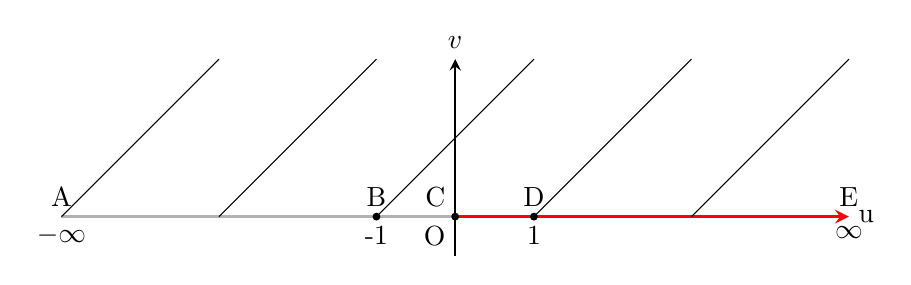
\begin{tikzpicture}
 \coordinate[label=below left:O] (O) at (0,0); %原点O
 \coordinate (XS) at (-5,0); %x軸最小
 \coordinate[label=right:u] (XL) at (5,0); %x軸最大
 \coordinate (YS) at (0,-0.5); %y軸最小
 \coordinate (YL) at (0,2); %y軸最大 
 \draw[very thick, white!70!black] (XS)--(O); %x軸
 \draw[very thick,->,>=stealth, red] (O)--(XL); %x軸
 \draw[thick,->,>=stealth] (YS)--(YL) node[above] {$v$}; %y軸
 \coordinate[label=above:D] (D) at (1, 0); %点z
 \coordinate[label=below:1] (D) at (1, 0); %点z
 \fill (D) circle (0.05); %zの塗りつぶし
 \coordinate[label=above left:C] (O) at (0, 0); %点z
 \fill (O) circle (0.05); %zの塗りつぶし
 \coordinate[label=above:B] (B) at (-1, 0); %点z
 \coordinate[label=below:-1] (B) at (-1, 0); %点z
 \fill (B) circle (0.05); %zの塗りつぶし
 \coordinate[label=above:A] (A) at (-5, 0); %点z
 \coordinate[label=below:$-\infty$] (A) at (-5, 0); %点z
 \coordinate[label=above:E] (E) at (5, 0); %点z
 \coordinate[label=below:$\infty$] (E) at (5, 0); %点z
 \draw (-5, 0)--(-3, 2);
 \draw (-3, 0)--(-1, 2);
 \draw (-1, 0)--(1, 2);
 \draw (1, 0)--(3, 2);
 \draw (3, 0)--(5, 2);
\end{tikzpicture}
\\

%(3)
\subsection{}
$$
\zeta = \xi + i\eta = \frac{1}{\pi}\mathrm{Log}{W} = \frac{1}{2\pi}\log{(u^2 + v^2)} + i\frac{1}{\pi}arg(w)
$$
点Aにおいては、
$$
\lim_{u \to -\infty, v \to 0}w = \infty + i\frac{1}{\pi} \times \pi = \infty + i
$$
点Bにおいては、
$$
\lim_{u \to -1, v \to 0}w = \frac{1}{2\pi}\log{1} + i\frac{1}{\pi} \times \pi = i
$$
点Cにおいては、
$$
 \lim_{\delta \to 0}\lim_{u \to \pm\delta, v \to 0}w =\begin{cases}
 \lim_{\delta \to 0}\mbox{\Large$\frac{1}{2\pi}$}\log{\delta} + i\frac{1}{\pi} \times \pi = -\infty + i\\
 \lim_{\delta \to 0}\mbox{\Large$\frac{1}{2\pi}$}\log{\delta} + i\frac{1}{\pi} \times 0 =- \infty 
 \end{cases}
$$
点Dにおいては、
$$
\lim_{u \to 1, v \to 0}w = \frac{1}{2\pi}\log{1} + i\frac{1}{\pi} \times 0 = 0
$$
点Eにおいては、
$$
\lim_{u \to \infty, v \to 0}w = \infty + i\frac{1}{\pi} \times 0 = \infty
$$
$-\infty \leq \xi \leq \infty$。また$0 \leq arg(w) \leq \pi$より、$0 \leq \eta \leq 1$\\
よって、$\zeta$の範囲は以下の斜線部分のようになる。\\
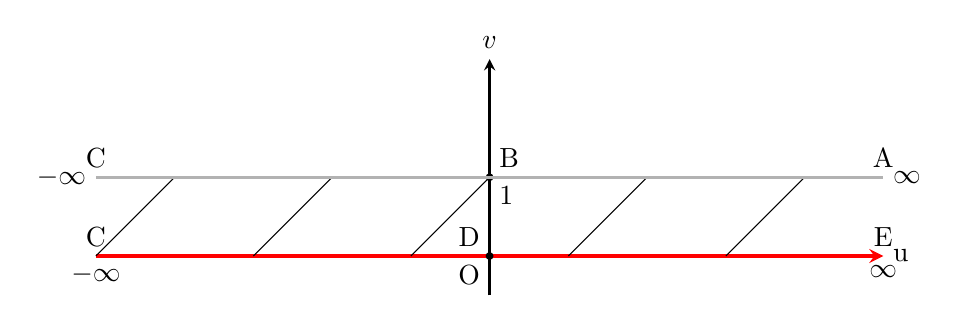
\begin{tikzpicture}
 \coordinate[label=below left:O] (O) at (0,0); %原点O
 \coordinate (XS) at (-5,0); %x軸最小
 \coordinate[label=right:u] (XL) at (5,0); %x軸最大
 \coordinate (YS) at (0,-0.5); %y軸最小
 \coordinate (YL) at (0,2.5); %y軸最大 
 \draw[very thick,->,>=stealth, red] (XS)--(XL); %x軸
 \draw[thick,->,>=stealth] (YS)--(YL) node[above] {$v$}; %y軸
 \coordinate[label=above right:B] (B) at (0, 1); %点z
 \coordinate[label=below right:1] (B) at (0, 1); %点z
 \fill (B) circle (0.05); %zの塗りつぶし
 \coordinate[label=above left:D] (O) at (0, 0); %点z
 \fill (O) circle (0.05); %zの塗りつぶし
 \coordinate[label=above:C] (C) at (-5, 0); %点z
 \coordinate[label=below:$-\infty$] (C) at (-5, 0); %点z
 \coordinate[label=above:A] (A) at (5, 1); %点z
 \coordinate[label=right:$\infty$] (A) at (5, 1); %点z
 \coordinate[label=above:C] (C_2) at (-5, 1); %点z
 \coordinate[label=left:$-\infty$] (C_2) at (-5, 1); %点z
 \coordinate[label=above:E] (E) at (5, 0); %点z
 \coordinate[label=below:$\infty$] (E) at (5, 0); %点z
 \draw (-5, 0)--(-4, 1);
 \draw (-3, 0)--(-2, 1);
 \draw (-1, 0)--(0, 1);
 \draw (1, 0)--(2, 1);
 \draw (3, 0)--(4, 1);
 \draw[very thick, white!70!black] (-5,1)--(5,1);
\end{tikzpicture}
\\

%(4)
\subsection{}
$\xi$方向には一定なので、
\begin{equation}
\label{3}
\partial_{\xi}T = 0
\end{equation}
$(\partial^2_{\xi} + \partial^2_{\eta})T = 0$、$\partial^2_{\xi}T = 0$より、$$\partial^2_{\eta}T = 0$$
よって、
\begin{equation}
\label{4}
\partial_{\eta}T = b \quad(b = const.)
\end{equation}
式(\ref{3})、式(\ref{4})から、
$$
T = a + b\eta
$$
境界条件$\eta = 1$の時$T = 1$、$\eta = 0$の時$T = 0$なので、
$$
T = \eta
$$

%(5)
\subsection{}
$$T(\xi, \eta) = \eta$$
$\eta = \mbox{\Large$\frac{1}{\pi}$}\mathrm{arctan}\mbox{\Large$\frac{v}{u}$}$より、
$$T(u, v) = \frac{1}{\pi}\mathrm{arctan}\frac{v}{u}$$
$w = i\mbox{\Large$\frac{1-z}{1+z}$}$より、
\begin{align*}
u + iv &= i\frac{1-x-iy}{1+x+iy}\\
&= i\frac{(1-x-iy)(1+x-iy)}{(1+x)^2 + y^2}\\
&= i\frac{(1-x-iy)(1+x-iy)}{(1+x)^2 + y^2}\\
&= i\frac{1-x^2-y^2-2iy}{(1+x)^2 + y^2}\\
&= \frac{2y + i(1-x^2-y^2)}{(1+x)^2 + y^2}\\
\therefore u = \frac{2y}{(1+x)^2 + y^2}&,\quad v =  \frac{1-x^2-y^2}{(1+x)^2 + y^2}
\end{align*}
よって、
\begin{align*}
T(x, y) &= \frac{1}{\pi}\mathrm{arctan}\frac{\frac{1-x^2-y^2}{(1+x)^2 + y^2}}{\frac{2y}{(1+x)^2 + y^2}}\\
&=\frac{1}{\pi}\mathrm{arctan}\frac{1-x^2-y^2}{2y}
\end{align*}
\\\\

%[3]
\section{主値積分}
略
\\\\

%[4]
\section{$\mbox{\Large$\int_{-\infty}^{\infty}$}R(x)\exp{(ix)}\mathrm{d}x$の積分}
$C_R$とは、半径Rの上半円を表すとする。
%(1)
\subsection{$\mbox{\Large$\int_{-\infty}^{\infty}\frac{x\sin{x}}{x^2 + a^2}$}\mathrm{d}x$}\begin{align*}
\int_{-\infty}^{\infty}\frac{x\sin{x}}{x^2 + a^2}\mathrm{d}x &= \Im\biggl[\int_{-\infty}^{\infty}\frac{ze^{iz}}{z^2 + a^2}\mathrm{d}z\biggr]\\
&= \Im\biggl[\oint_C\frac{ze^{iz}}{z^2 + a^2}\mathrm{d}z\biggr]\quad(Cは以下の図の積分経路\because ジョルダンの補題)\\
&= \Im\biggl[\frac{1}{2}\oint_C\Bigl(\frac{1}{z-ia}+\frac{1}{z+ia}\Bigr)e^{iz}\mathrm{d}z\biggr]\\
&= \frac{1}{2}\Im\biggl[\oint_C\frac{1}{z-ia}e^{iz}\mathrm{d}z\biggr]\quad(\because z = -iaは積分経路外)\\
&= \frac{1}{2}\Im\biggl[2\pi i\times Res\Bigl(\frac{e^{iz}}{z-ia}, z = ia\Bigr)\biggr]\\
&= \frac{1}{2}\biggl[2\pi i\times e^{-a}\biggr]\\
&= \pi e^{-a}
\end{align*}
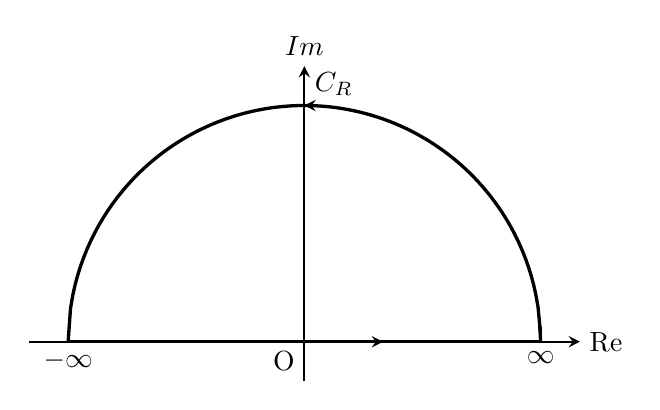
\begin{tikzpicture}
 \coordinate[label=below left:O] (O) at (0,0); %原点O
 \coordinate (XS) at (-3.5,0); %x軸最小
 \coordinate[label=right:Re] (XL) at (3.5,0); %x軸最大
 \coordinate (YS) at (0,-0.5); %y軸最小
 \coordinate (YL) at (0,3.5); %y軸最大 
 \draw[thick,->,>=stealth] (XS)--(XL); %x軸
 \draw[thick,->,>=stealth] (0,0)--(1,0); %x軸
 \draw[thick,->,>=stealth] (0.001,3)node[above right] {$C_R$}--(0,3); %x軸
 \draw[thick,->,>=stealth] (YS)--(YL) node[above] {$Im$}; %y軸
 \draw[very thick] [samples = 200, domain=-3:3] plot(\x, {sqrt(9 - (\x) ^2 )});
 \draw[very thick] (-3,0)--(3,0); %x軸
 \draw[very thick] (3,0)--(2.99,0.2); 
 \coordinate[label=below: $\infty$] (A) at (3,0); %点z
 \coordinate[label=below: $-\infty$] (B) at (-3,0); %点z
\end{tikzpicture}

%(2)
\subsection{}
略\\

%(3)
\subsection{$\mbox{\Large$\int_{-\infty}^{\infty}\frac{\sin{x}}{x}$}\mathrm{d}x$}
\begin{align*}
\int_{-\infty}^{\infty}\frac{\sin{x}}{x}\mathrm{d}x &= \Im\biggl[\int_{-\infty}^{\infty}\frac{e^{iz}}{z}\mathrm{d}z\biggr]\\
&= \Im\biggl[\oint_{C}\frac{e^{iz}}{z}\mathrm{d}z - \lim_{\delta \to 0}\int_{C_{\delta}}\frac{e^{iz}}{z}\mathrm{d}z\biggr]\quad(\because ジョルダンの補題)\\
&= \Im\biggl[- \lim_{\delta \to 0}\int_{C_{\delta}}\frac{e^{iz}}{z}\mathrm{d}z\biggr]\quad(\because \frac{e^{iz}}{z}は積分経路内に極を含まないので周回積分は0)\\
&= \Im\biggl[- \lim_{\delta \to 0}\int_{C_{\delta}}\frac{1}{z}(1 + iz -z^2 -iz^3 +\cdots)\mathrm{d}z\biggr]\\
&= -\lim_{\epsilon \ to 0} \Im\biggl[\int_{\pi}^{0}\frac{1}{\epsilon^{i\theta}}(1 + i\epsilon e^{i\theta} -\epsilon e^{2i\theta} -i\epsilon e^{3i\theta} +\cdots)i\epsilon e^{i\theta}\mathrm{d}\theta\biggr]\\
&= \lim_{\epsilon \ to 0} \int_{0}^{\pi}(1 -\epsilon e^{2i\theta} -\cdots)\mathrm{d}\theta\\
&= \pi
\end{align*}
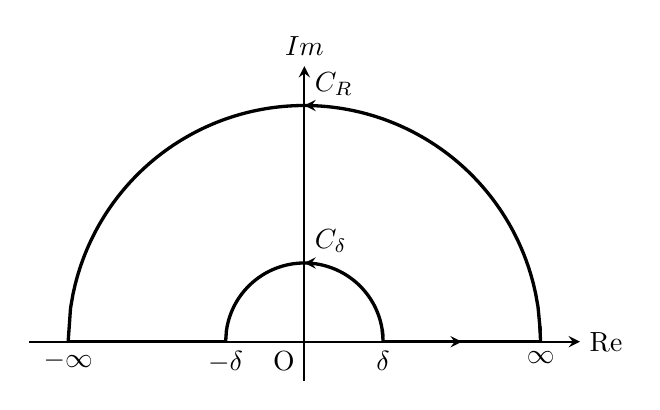
\begin{tikzpicture}
 \coordinate[label=below left:O] (O) at (0,0); %原点O
 \coordinate (XS) at (-3.5,0); %x軸最小
 \coordinate[label=right:Re] (XL) at (3.5,0); %x軸最大
 \coordinate (YS) at (0,-0.5); %y軸最小
 \coordinate (YL) at (0,3.5); %y軸最大 
 \draw[thick,->,>=stealth] (XS)--(XL); %x軸
 \draw[thick,->,>=stealth] (0,0)--(2,0); %x軸
 \draw[thick,->,>=stealth] (0.001,3)node[above right] {$C_R$}--(0,3); 
 \draw[thick,->,>=stealth] (0.001,1)node[above right] {$C_{\delta}$}--(0,1);
 \draw[thick,->,>=stealth] (YS)--(YL) node[above] {$Im$}; %y軸
 \draw[very thick] [samples = 200, domain=-3:3] plot(\x, {sqrt(9 - (\x) ^2 )});
 \draw[very thick] [samples = 200, domain=-1:1] plot(\x, {sqrt(1 - (\x) ^2 )});
 \draw[very thick] (-3,0)--(-1,0);
 \draw[very thick] (1,0)--(3,0);
 \draw[very thick] (3,0)--(2.99,0.2); 
 \draw[very thick] (1,0)--(0.99,0.15); 
 \coordinate[label=below: $\infty$] (A) at (3,0); %点z
 \coordinate[label=below: $-\infty$] (B) at (-3,0); %点z
 \coordinate[label=below: $\delta$] (A) at (1,0); %点z
 \coordinate[label=below: $-\delta$] (B) at (-1,0); %点z
\end{tikzpicture}
\\\\

%[5]
\section{Cauchy主値}
%(1)
\subsection{$P_v\mbox{\Large$\int_{-\infty}^{\infty}\frac{1}{(x^2+1)(x-a)}$}\mathrm{d}x$}
\begin{align*}
P_v\int_{-\infty}^{\infty}\frac{1}{(x^2+1)(x-a)}\mathrm{d}x &= 2\pi i Res\Bigl(\frac{1}{(x^2+1)(x-a)}, i\Bigr) + \pi i Res\Bigl(\frac{1}{(x^2+1)(x-a)}, a\Bigr)\\
&= 2\pi i\frac{1}{2i(i-a)} + \pi i\frac{1}{a^2+1}\\
&= -\frac{\pi a}{a^2+1}
\end{align*}
\\

%(2)
\subsection{$P_v\mbox{\Large$\int_{-\infty}^{\infty}\frac{1}{x(x^2 -x + 1)}$}\mathrm{d}x$}
\begin{align*}
P_v\int_{-\infty}^{\infty}\frac{1}{x(x^2 -x + 1)}\mathrm{d}x &= 2\pi i Res\Bigl(\frac{1}{x(x^2 -x + 1)}, \frac{1 + i\sqrt{3}}{2}\Bigr) + \pi i Res\Bigl(\frac{1}{x(x^2 -x + 1)}, 0\Bigr)\\
&= 2\pi i\frac{1}{\frac{1 + i\sqrt{3}}{2}i\sqrt{3}} + \pi i\\
&= \frac{\sqrt{3}}{3}\pi
\end{align*}
\\

%(3)
\subsection{$P_v\mbox{\Large$\int_{-\infty}^{\infty}\frac{1}{x+2} - \frac{1}{x-2}$}\mathrm{d}x$}
\begin{align*}
\int_{-\infty}^{\infty}\frac{1}{x+2} - \frac{1}{x-2}\mathrm{d}x &= \pi i Res\Bigl(\frac{1}{x+2}, -2\Bigr) - \pi i Res\Bigl(\frac{1}{x-2}, 2\Bigr)\\
 &= \pi i - \pi i\\
 &= 0
\end{align*}
\\

%(4)
\subsection{$P_v\mbox{\Large$\int_{-\infty}^{\infty}\frac{1}{x-a} + \frac{1}{x-b} - \frac{2}{x}$}\mathrm{d}x$}
\begin{align*}
\int_{-\infty}^{\infty}\frac{1}{x-a} + \frac{1}{x-b} - \frac{2}{x}\mathrm{d}x &= \pi i Res\Bigl(\frac{1}{x-a}, a\Bigr) + \pi i Res\Bigl(\frac{1}{x-b}, b\Bigr) + \pi i Res\Bigl(\frac{2}{x}, 0\Bigr)\\
 &= \pi i + \pi i - 2\pi i\\
 &= 0
\end{align*}

\end{document}